\documentclass[dvipdfmx,cjk,t,10pt]{beamer}  
%\documentclass[cjk,t]{beamer}


\usepackage{kasailab_slide_def}
\usepackage{color}
\usepackage{lastpage}
\usepackage{amssymb,bbm}
\usepackage{subfigure}
\setbeamertemplate{footline}[text line]{%
  \parbox{1.00\linewidth}{
    \vspace*{-8pt}\hspace*{-20pt}\textcolor{gray}{KASAI Laboratory, WASEDA University. All Rights Reserved.}}
  \hfill%
  \parbox{0.07\linewidth}{
    \vspace*{-8pt} \hfill \textcolor{gray}{\raggedright\insertpagenumber /{}\pageref{LastPage}}
  }
} 

%%目次スライド 
% 研究進捗では使用しないこと
%\AtBeginSection[]{
%    \frame{\tableofcontents[currentsection, hideallsubsections]} 
%}


%%%%%%%%%%%%%%%%%%%%%%%%%%%%%%%%%%%%%%%%%%%%%%%%%%%%%%%%%%%%%%%%%%%%%%%%%%
\newcommand{\x}{\mathbf x}
\newcommand{\y}{\mathbf y}
\newcommand{\C}{\mathbf C}
\newcommand{\T}{\mathbf T}
\newcommand{\calC} {\mathcal{C}}
\newcommand{\bfP} {\mathbf{P}}
\newcommand{\kl}{\mathbf {KL}}
\newcommand{\kll}{\mathcal {KL}}
\newcommand{\OTmp}[1]{\hat{\mathbf{P}}_{#1}}
\newcommand{\prox}{\operatorname{prox}}
\newcommand{\proj}{\operatorname{Proj}}
\newcommand{\diag}{\operatorname{diag}}
\newcommand{\argmin}{\operatorname{argmin}}
\newcommand{\tranT}{\mathsf T}

%%%%%%% TITLE PAGE %%%%%%%%%%%%%%%%%%%%%%%%%%%%%%%%%%%%%%%%%%%%%%%%%%%


\begin{document}

\title{Mirror Descent on Unbalanced Optimal Transport and Acceleration}

%\author{Hiroyuki }
\author[shortname]{Su Xun}
\institute[shortinst]{笠井研究室 修士2年}
%\date{2019年5月15日}

\begin{frame}
\titlepage
	
	\vspace*{-0.5cm}
\end{frame}

\section{Outline}
\begin{frame}
\frametitle{Outline}
%\framesubtitle{sub title}

	\begin{itemize}
	\item Backgrounds of Optimal Transport and Unbalanced Optimal Transport problems
	\itemspace	
	\item The Lasso problem and Mirror Descent Algorithms
	\itemspace	
	\item Acceleration 
	\itemspace	
	\item Shifting projection
	\itemspace
	\item Prospect and Plan
	\itemspace
	\end{itemize}		
\end{frame}


\section{Backgrounds}
\begin{frame}
	\begin{screen}{Optimal Transport}
$$
\begin{aligned}
&W(\alpha,\beta) := \min_{ \mathbf{T} \in \mathbb{R}_{+}^{n \times n}} \langle \C, \mathbf{T} \rangle \\
& \mathbf{T} \mathbbm{1} = \alpha, \mathbf{T}^{T}\mathbbm{1} = \beta, \mathbf{T}_{ij}>0
\end{aligned}
$$
\end{screen}	
	\begin{itemize}
	\item Applications on GAN, Retrieving information, Domain adaptation, and so on.
	\end{itemize}	
	\begin{figure}[htbp]
	\begin{center}	
	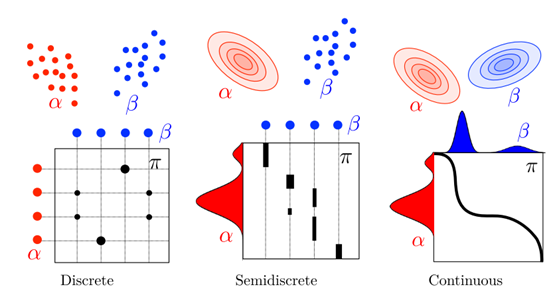
\includegraphics[width=0.5\hsize]{pic/ot}
	\caption{Different forms of Optimal Transport}
	\end{center}	
	\end{figure}			
	
\end{frame}


\begin{frame}
	\begin{screen}{Unbalanced Optimal Transport (UOT)}
$$
W(\alpha,\beta) := \min_{ \mathbf{T} \in \mathbb{R}_{+}^{n \times n}} \langle \C, \mathbf{T} \rangle + \tau D_h(\mathbf{T} \mathbbm{1},\alpha)+\tau D_h( \mathbf{T}^{T}\mathbbm{1},\beta)
$$

\end{screen}
	
	\begin{itemize}
	\item Optimal Transport can only deal with balanced samples, a relaxed version with divergence function $D_h$ is required for more general applications.
	\item the most famous UOT solver is the Sinkhorn, which uses Kullback-Leibler divergence to penalize and add an entropy part $\eta H(\mathbf{T})$ onto the problem, its complexity is $O(\frac{n^2}{\epsilon})$ $\cite{DBLP:journals/corr/abs-2002-03293}$
	\item It is natural to consider whether other powerful optimizers exist.
	\end{itemize}
\end{frame}


\section{Algorithms}
\begin{frame}
\frametitle{Lasso problem and Mirror Descent }
	
	\begin{itemize}
	\item UOT has a similar structure to the Lasso problem:
$$
\begin{aligned}
f(t) = g(t) + D_h(Xt,b), t\in \mathbbm{R}^{n^2}
\end{aligned}
$$
\item Lasso Problem:
$$
\begin{aligned}
f(t) = \lambda\|t\| + \|Xt-b\|_2^2
\end{aligned}
$$
\item $L_2$ or Kullback-Leibler divergence penalized UOT
$$
\begin{aligned}
f(t) &= \lambda c^{\tranT}t + \|Xt-b\|_2^2\\
f(t) &= \lambda c^{\tranT}t + KL(Xt,b)
\end{aligned}
$$
$b=[\alpha^{\tranT} \quad \beta^{\tranT}]^{\tranT}$ and $X$, for example, when $n=3$, is:
\begin{align}
 X= 
\begin{pmatrix}
1&1&1& & & & & &\\
 & & &1&1&1& & &\\
 & & & & & &1&1&1\\
1& & &1& & &1& &\\
 &1& & &1& & &1&\\
 & &1& & &1& & &1\\
\end{pmatrix}
\end{align}	
\end{itemize}
\end{frame}




\begin{frame}
\frametitle{Lasso problem and Mirror Descent }
	The problem with a similar structure is suitable for Mirror Descent Algorithm. 
		\begin{screen}{Composite convex problem}
$$
\min _{x \in \mathbb{R}^{n}}\{d(x)+g(x)\}
$$
$d(x)$ is convex and differentiable and $g(x)$ is convex.
	\end{screen}	

\begin{itemize}
	\item Proximal Gradient
	$$
\operatorname{Prox}_{\gamma}(x):=\underset{z \in \mathbb{R}^{n}}{\operatorname{argmin}}\left\{\frac{1}{2 \gamma}\|z-x\|^{2}+g(z)\right\}
$$
	\item Bregman Proximal
	$$
\operatorname{Prox}_{\gamma}(x):=\underset{z \in \mathbb{R}^{n}}{\operatorname{argmin}}\left\{\frac{1}{2 \gamma}D_h(z,x)+g(z)\right\}
$$
	
\end{itemize}
\end{frame}


\begin{frame}
\frametitle{Lasso problem and Mirror Descent}
		\begin{screen}{Composite convex problem}
$$
\min _{x \in \mathbb{R}^{n}}\{d(x)+g(x)\}
$$
	\end{screen}	
\begin{itemize}
	\item For Lasso:
	$$
		d(x)= \|At-b\|_2^2, \quad g(x) = \lambda \|t\|
	$$
	
	\item For $L_2$ penalized UOT:
	$$
		d(x)= \|At-b\|_2^2, \quad g(x) = \lambda c^{\tranT}t
	$$

	\item For Kullback-Leibler divergence penalized UOT:
	$$
		d(x)= KL(At,b),\quad g(x) =  \lambda c^{\tranT}t
	$$
\end{itemize}

\end{frame}

\begin{frame}
\frametitle{Lasso problem and Mirror Descent}
\begin{itemize}
\item For $L_2$ UOT, we get
$$
 T^{k+1} = \max(T^{k} -\gamma (T^{k}\mathbbm{1}\mathbbm{1}^{\tranT}+\mathbbm{1}\mathbbm{1}^{\tranT}T^{k})-\alpha\mathbbm{1}^{\tranT}+\mathbbm{1}\beta^{\tranT}-\lambda \C,0)
$$
It is the ISTA algorithm. 
\item For $KL$ UOT, we get
$$
T_{k+1}= (\diag{(\frac{\alpha}{T_k\mathbbm{1}})})^{\gamma}(T_k\odot \exp{(-\gamma \lambda \C)})(\diag{(\frac{\beta}{T_k^{\tranT}\mathbbm{1}})})^{\gamma} 
$$
when $\gamma = \frac{1}{L} = \frac{1}{2}$ ($f(x)$ is an $L$-strongly convex function), it is equal to the Majorization-Minimization (MM) algorithm in $\cite{https://doi.org/10.48550/arxiv.2106.04145}$.
\end{itemize}
\end{frame}

\section{Accelerations}
\begin{frame}
\frametitle{Acceleration Methods}
		\begin{itemize}
		\item   Lucky, we can borrow the accelerating methods from the Lasso problem:
		\begin{itemize}
		\item  Nesterov Acceleration
		\item  Path-following Algorithm \cite{Tibshirani_2011}
		\item  Screening \cite{ghaoui2010safe}
	   	\end{itemize}
	   	\item  I am focusing on the Screening method and I revised this method for the UOT problem to take advantage of its sparse $X$ matrix, which is rare in the normal Lasso problem. 

	   	\end{itemize}

\end{frame}





\begin{frame}
\frametitle{Screening}
	\begin{screen}{Motivation:}
	
	\quad Lasso-like regularizations cause a sparse solution $\operatorname{card}(t_{ij}\|t_{ij} = 0)\approx n^2$, for $t \in \mathbb{R}^{n \times n}$. We identify the elements equal to zero theoretically and freeze them to save computational time.
	
	\end{screen}	
		\begin{itemize}
		\item As the UOT could be regarded as a Lasso-like problem, this technology can handle UOT as well.
	   	\end{itemize}
	\begin{figure}[htbp]
	\begin{center}	
	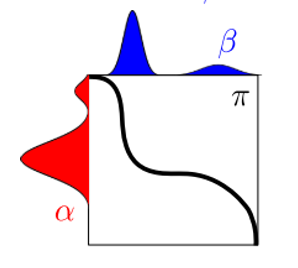
\includegraphics[width=0.3\hsize]{pic/sparse}
	\caption{The typical sparse solution for OT problem}
	\end{center}	
	\end{figure}	
	
\end{frame}


\begin{frame}
\frametitle{Screening}
	\begin{screen}{Dynamic Screening Framework \cite{NEURIPS2021_7b5b23f4}}
	$$
	P(t) = \min_{t} d(Xt) + g(t)
	$$
	$$
	D(\theta) = \max_{\theta} -d^{*}(-\theta) + g^{*}(X^{T}\theta)
	$$
	\end{screen}	
		\begin{itemize}
		\item $d(Xt)$ is the distance measure like $L_2$ function and KL divergence.
		\item $g(\beta)$ is the Lasso-like sparse regularization such as $L_1$ penalty or optimal transport problem, we can convert it to constraints, then the dual problem is:  
	\end{itemize}
			$$
	\begin{aligned}
			&D(\theta) =  \max_{\theta}-d^{*}(-\theta)\\
			&\text{s.t.}\quad \forall i,\quad  h_{i}(\theta)\leq 0\\  
	\end{aligned}
		$$
\end{frame}

\begin{frame}
\frametitle{Screening}	
		\begin{itemize}
		 \item Relying on the KKT condition, we can assert the existence of a series of dual constraints $h_{i}(\theta)$, that for optimum $\hat{\theta}$, if $h_{i}(\hat{\theta})<0$, then $t_i=0$. 
		 \item For Lasso, the dual constraints are: 
		$$
		{h_{i}(\theta)=\|x_i^{T}\theta\| - 1 \leq 0} 
		$$
		\item For UOT, the dual constraints are: 
		$$
		{h_{i}(\theta)=x_i^{T}\theta - c_i \leq 0} 
		$$
		\item For $\hat{\theta}$, if the the $\leq$ could be replaced by $<$, then  we have ${\hat{t_{i}}} = 0$
		\item However, we don't know the value of the optimum solution $\hat{\theta}$ at first.
		\end{itemize}
\end{frame}


\begin{frame}
\frametitle{Screening}	
		\begin{itemize}
		\item If we can find a $\tilde{\theta}$ that satisefied with the dual constrains, then we can construct an area $R^{DS}(\tilde{\theta})$, for $L_2$ penalized problem:
		$$
	\begin{aligned}
	&\frac{1}{2}\| \theta -\tilde{\theta}\|_2^{2} + D(\tilde{\theta}) \leq D(\theta) \leq -d^{*}(-\theta) \\
	& \text{s.t. } g(\tilde{t})-\theta^{T}X\tilde{t}< 0
	\end{aligned}
	$$
		\item The left part is strongly concave inequality and the right part is the dual inequality. 
		\item This area contains $\tilde{\theta}$ and the optimum $\hat{\theta}$
		\item If we could prove the $\max_{\theta \in R^{DS}(\tilde{\theta}) } h_{i}(\theta)<0$, then it holds for the optimum $\hat{\theta}$. It indicates that $ h_{i}(\hat{\theta})<0$, and the element $i$ of the primal optimal solution $\hat{t}$ must be zero. 
		\end{itemize}
\end{frame}


\begin{frame}
\frametitle{Screening}
	\begin{figure}[htbp]
	\begin{center}	
	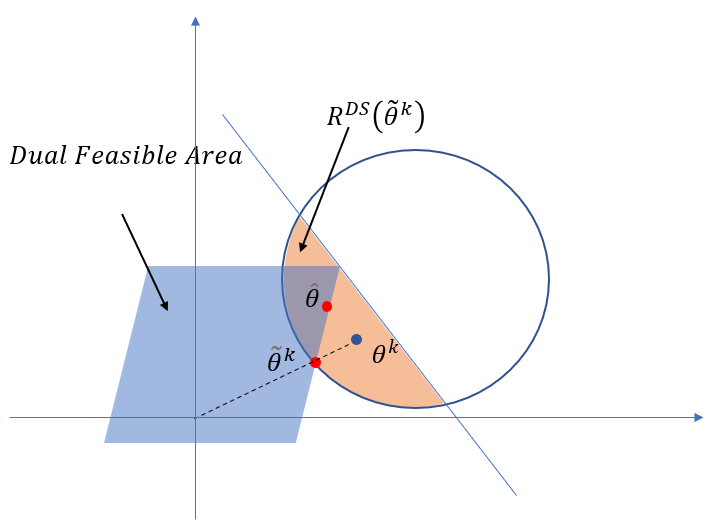
\includegraphics[width=0.8\hsize]{pic/proj}
	\caption{Projection in Screening}
	\end{center}	
	\end{figure}	
\end{frame}


\begin{frame}
\frametitle{Screening}
	\begin{itemize}
		\item We can dynamically compute an approximate solution $\theta^{k}$ by any algorithm and project it onto the dual constraints as $\tilde{\theta}^{k}$.
		\item We hope the projected $\tilde{\theta}^{k}$ could be closed enough to $\hat{\theta}$ to produce a smaller $R^{DS}(\tilde{\theta}^{k})$
		\item A smaller area can help us screen more variables as 
		$$
		\max_{\theta \in \tilde{R} \in R^{DS}(\tilde{\theta})}{\|x_i^{T}\theta\|} \leq \max_{\theta \in R^{DS}(\tilde{\theta})}{\|x_i^{T}\theta\|} 
		$$
		always holds.

	\end{itemize}
	
\end{frame}


\begin{frame}
\frametitle{Projection methods}
	\begin{itemize}
		\item The Lasso method is to shrink all $\tilde{\theta}$ together.
		$$
			\tilde{\theta} = \frac{\theta}{\|\frac{X^{T}\theta}{c}\|_{\infty}}
		$$
	
		\item It is not suitable for the UOT problem as the cost value $c_{i}$ might be small and even zero. 
		\item We propose to use a shifting method, as the $x_{i}$ has a specific sparse structure which could rewrite the problem as:
		$$
		\theta_{i_{1}}+\theta_{i_{1}}<c_i
		$$
		we decide to shift $\theta_{j}$ according to the maximum positive difference of $	\frac{\theta_{i_{1}}+\theta_{i_{1}}-c_i}{2}$
	\end{itemize}
\end{frame}


\begin{frame}
\frametitle{Screening}
Shifting Screening method:
		$$
		\tilde{\theta}_{i}=\left\{
	\begin{aligned}
			\theta_{i} - \max_{j \mod n =i}(\frac{\theta_{j_{1}}+\theta_{j_{2}}-c_j}{2}) &\quad 0\leq i<n\\
			\theta_{i} - \max_{in\leq j <i(n+1)}(\frac{\theta_{j_{1}}+\theta_{j_{2}}-c_j}{2}) & \quad n\leq i<2n
	\end{aligned}
	\right.
		$$
	\begin{figure}[htbp]
	\begin{center}	
	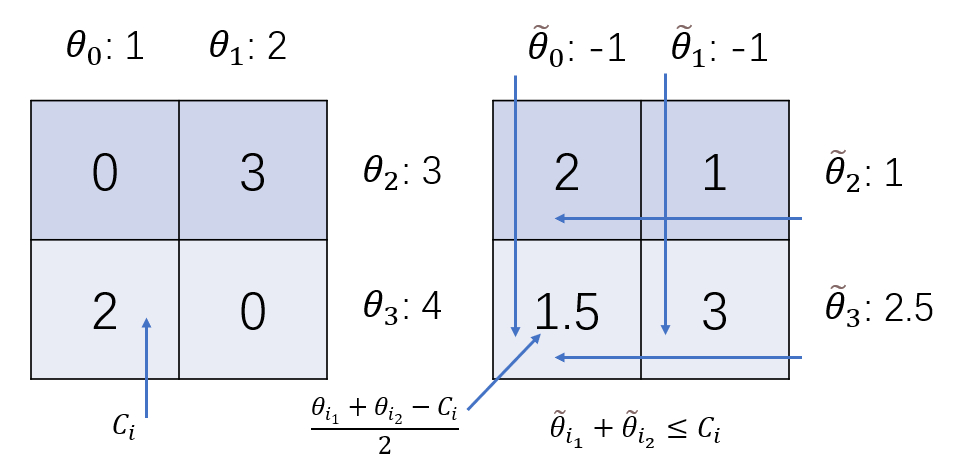
\includegraphics[width=0.8\hsize]{pic/shifting}
	\caption{Shifting on a 2$\times$2 matrix}
	\end{center}	
	\end{figure}

\end{frame}

\begin{frame}
\frametitle{Screening}
	\begin{figure}[htbp]
	\begin{center}	
	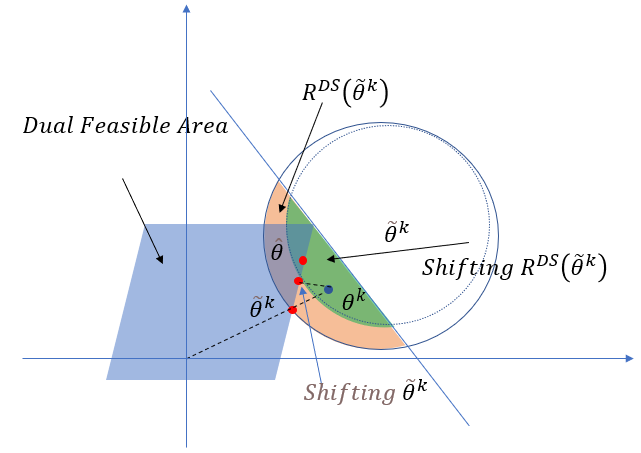
\includegraphics[width=0.8\hsize]{pic/new_proj}
	\caption{Difference of the projection method in Screening}
	\end{center}	
	\end{figure}

\end{frame}


\begin{frame}
\frametitle{Screening}
	\begin{figure}[htbp]
	\begin{center}	
	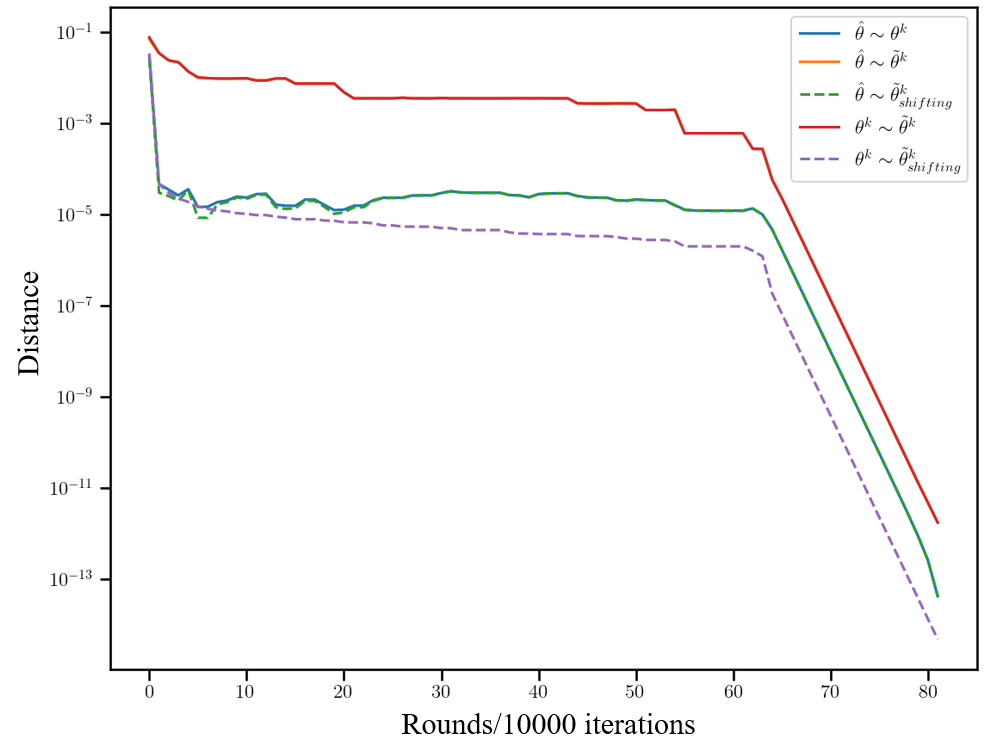
\includegraphics[width=0.8\hsize]{pic/dis}
	\caption{Distance between the projected point with $\hat{\theta}$ or $\theta^k$ }
	\end{center}	
	\end{figure}

\end{frame}

\begin{frame}
\frametitle{Screening}
	\begin{figure}[htbp]
	\begin{center}	
	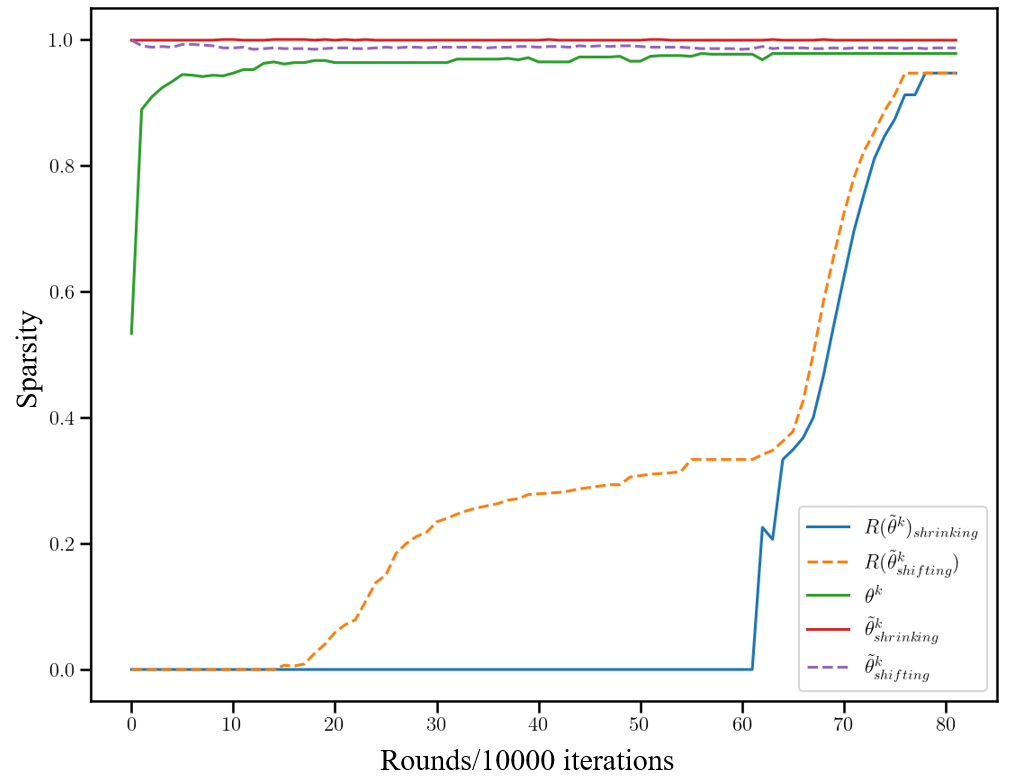
\includegraphics[width=0.8\hsize]{pic/spa}
	\caption{The Screening Ratio}
	\end{center}	
	\end{figure}

\end{frame}


\section{Prospect and Plan}
\begin{frame}
\frametitle{Potential and defects}
	\begin{itemize}	
	\item The UOT problem has the potential to screen out better due to its specific sparse structure of matrix $X$
	\item Screening is irrelevant to the optimization method you use and especially effective for the MM algorithm (which could be regarded as one kind of Mirror Descent)
	\item KL penalized Lasso problem also has a screening method \cite{9414183}, which could be applied to the KL penalized UOT problem, we might accelerate Sinkhorn Algorithm, which is only suitable for KL penalized UOT, with the Screening method.
	\item However, Screening needs too many iterations to start even after the revision. There might exist a better method to find a smaller area for the UOT problem
	\end{itemize}	
\end{frame}

\begin{frame}
\frametitle{Future Plan}
	\begin{itemize}
	\item Thinking of revising the screening method from the perspective of constructing area.
	\item Combining the Screening method with Mirror descent and other algorithms to test its speed-up ratio.
	\item Generalizing the screening method to KL penalized the UOT problem and the Sinkhorn Algorithm.  
	\end{itemize}	
\end{frame}

\section{Reference}

\begin{frame}[allowframebreaks]
%\setbeamertemplate{bibliography item}[text]
\setbeamertemplate{bibliography item}[triangle]
        \frametitle{References}
        %\bibliographystyle{amsalpha}
        \bibliographystyle{apalike}
        \bibliography{sample}
\end{frame}


\begin{frame}
	\begin{center}	
	\vspace*{1.0cm}
	\IMPB{\Large ご清聴ありがとうございました. }	
	
	\vsp\vsp
	\IMPB{\Large Thank you for listening. }
	\vspace*{1.0cm}
	\end{center}	
	\vspace*{-0.5cm}
\end{frame}

\end{document}





